\scanpage{59}
Catégories de Deuring.

1. Catégories $A$-linéaires et $\otimes$-enveloppes.

$A$ est un annea\unsure{\deleted{t}u|\deleted{u}t} commutatif. Soit $C$ une catégorie $A$-linéaire (i.e. les $\operatorname{Hom}$ dans $A$ sont des $A$-modules, l'accouplement des $\operatorname{Hom}$ étant bilinéaire). Un \unsure{\deleted{h}f|\deleted{f}h}oncteur $A$-linéaire
\[
F:\ C\handwritten{\longrightarrow}C'
\]
de $C$ dans une autre catégorie $A$-linéaire $C'$ est dit \inserted{``admissible'' ou} ``compatible au produit tensoriel externe'' si pour tout objet $X$ de $C$ sur lequel opère ($A$-linéairement) une $A$-algèbre $o$, et tout $o$-module à droite $P$ tel que $P\otimes_o X$ existe dans $C$, $\deleted{\unsure{F(}}P\deleted{)}\otimes_o F(X)$ existe dans $C'$ et l'homomorphisme naturel
\margin{\figure{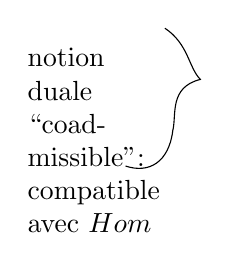
\begin{tikzpicture}[x=1cm,y=1cm]
\node[anchor=north west,text width=1.7cm,inner sep=0pt] at (0,0) {notion duale ``coadmissible'': compatible avec $\operatorname{Hom}$};
\handwritten{\draw (1.75,.25) .. controls (2.05,.05) and (2.05,-.25) .. (2.2,-.4) .. controls (1.8,-.5) and (1.9,-.85) .. (1.85,-1.05) .. controls (1.8,-1.45) and (1.55,-1.6) .. (1.25,-1.5);}
\end{tikzpicture}}}
\[
P\otimes_o F(X)\handwritten{\unsure{\text{---}|\longrightarrow}}F(P\otimes_o X)
\]
est un isomorphisme. Si $C$ est une catégorie de Deuring, alors il suffit de poser cette condition pour un objet fixé $X$ de $C$, et pour $o=\operatorname{End}_C(X)$, $P$ un module $\handwritten{\in}\uline{P}(\handwritten{o/A})=$ catégorie des $o$-modules à droite qui sont localement sur $S=\operatorname{Spec}(A)$ libres de rang $1$. Dans ce cas, la catégorie des foncteurs $F$ en question est équivalente, par
\margin{\handwritten{il suffit que $C$ admette $X$ \deleted{\unsure{comme|un}} ``générateur strict'' i.e. tt objet de $C$ de la forme $P\otimes_o X$, et que avec $P$ projectif de type fini, alors équiv. $\uline{P}\longmapsto P\otimes_o X$ (sur ss-cat $\unsure{\mathbb{P}(o)X|P(o)X}$) (pour $P\otimes_o X$ \unsure{existe})}}
\margin{\handwritten{$P\otimes_o X\overset{\sim}{\longrightarrow}\operatorname{Hom}_o(\check P,X)$}}
\[
F\handwritten{\longmapsto}F(X)\ :\ \uline{\operatorname{Hom}}_{A\text{-}\mathrm{adm}}(C,C')\handwritten{\hookrightarrow}\operatorname{Mod}(o,C'),
\]
à la catégorie des objets \inserted{$X'$} de $C'$ avec opération de $o$\inserted{$A$-linéaire de}, tels que $P\otimes_o X'$ exist dans $C'$ pour tout $P\handwritten{\in}\operatorname{ob}\uline{P}(o/A)$. En tous cas, la catégorie des foncteurs admissibles de $C$ dans $C'$ est $A$-linéaire.

\inserted{Soit}
\[
\deleted{\text{Soit}}\quad C(1)=\uline{\operatorname{Hom}}_{A\deleted{\text{-}\mathrm{adm}}\inserted{\handwritten{\mathrm{coadm}}}}(C^{\handwritten{\unsure{o|0|\circ}}},\operatorname{Mod}(A)),
\]
on a alors un foncteur pleinement fidèle canonique
\[
C\handwritten{\xrightarrow{i}}C(1)
\]
associant à tout objet $X$ de $C$ le foncteur $Y\handwritten{\longmapsto}\operatorname{Hom}_{\mathbb{C}}(Y,X)$ qu'il représente. \handwritten{Si $X$ est un objet de $C$ tel que tout objet \inserted{$Y$} de $C$ s'écrit sous la forme $P\otimes_o X$, avec $P$ un $o$-module à droite projectif de type fini $(o=\operatorname{End}_C(\unsure{X^{\prime}|X}))$.}
% archive sheet number: 58
